% This is samplepaper.tex, a sample chapter demonstrating the
% LLNCS macro package for Springer Computer Science proceedings;
% Version 2.20 of 2017/10/04
%
\documentclass[runningheads]{llncs}
%
\usepackage{graphicx}
% Used for displaying a sample figure. If possible, figure files should
% be included in EPS format.
%
% If you use the hyperref package, please uncomment the following line
% to display URLs in blue roman font according to Springer's eBook style:
% \renewcommand\UrlFont{\color{blue}\rmfamily}

\begin{document}
%
\title{Nationwide Amtrak Rail Performance}
%
%\titlerunning{Abbreviated paper title}
% If the paper title is too long for the running head, you can set
% an abbreviated paper title here
%
\author{Edward Harianto \and
Soumeya Kerrar \and
Sandra Rajoo \and Winston Zhou}
%
% First names are abbreviated in the running head.
% If there are more than two authors, 'et al.' is used.
%
\institute{University of Southern California, Los Angeles, CA 90007, USA}
%
\maketitle              % typeset the header of the contribution
%
%
%
%
\section{Introduction and Background}
Long distance and high speed travel by rail has been a persistent issue in the transportation sector in the United States. With connectivity lacking between major hubs, and a disparity of Amtrak stations in certain parts of the country, transportation reform often looks to improve travel access in the country in modes that don’t include automobile or air travel. By 2035, Amtrak aims to make significant changes in order to address the continued issue of unmet demand for rail travel and a need for increase in reliable and efficient rail service in the nation~\cite{url}. In this project, we explore various aspects of the performance of Amtrak’s trains, as the nation’s only nationwide railroad company. The aim is to provide a visual representation of delays, routes and ridership, which can inform Amtrak staff and leadership on railroad improvements, funding needs and infrastructure improvements. The dashboard contains an interactive map which allows for predicting the delay between stations. Further charts display the top busiest stations by ridership, average delay per station, performance of the trains, and on time performance. Increasing on time performance is essential in order for Amtrak to become lucrative, rather than be losing funds as has been shown in the past. The dashboard was created with the vision in mind that the user would be involved in Amtrak decision making, and therefore offers various tools that can inform these decisions. It can also be of use to an average rider who is interested in knowing how this mode of access performs, especially in comparison to other modes they may consider.  

\section{Design and Development}
In order to meet our goals, data was collected from Amtrak for ridership information and from the archive at dixielandsoftware.net for performance, arrival, departure, and delay data. Both sets of data were cleaned and processed in order to implement the different components of our dashboard. The elements of our dashboard were created using D3 for charts, Mapbox for the dynamic map and Python for the predictive model performance. The project was integrated using the Vue framework.

\section{Predictive Model}
A model was built to predict Amtrak trains’ delays along trains between different stations. It also offers the probability of arriving at the destination at different times. The model was built using a dataset of 8 variables: Train Number, Origin Date, Station, Arrival/Depart (i.e., whether the row corresponds to a train arriving or departing), Scheduled Time, Actual Time, Difference, and Trip Day (the day of the trip the train made it to the row’s station). The engineered feature used in the model is the difference between the actual and scheduled departure or arrival at a given station. The purpose of creating a predictive model is to allow the end user to estimate delays and address on-time performance of Amtrak trains.

\section{Dashboard}
\subsection{Route Analysis}
\subsubsection{Mapbox Map}
The chart below shows a Mapbox map of the Amtrak Routes. The purpose of this map is to allow users to visualize all the possible locations that an Amtrak train will go through in the United States.
\begin{figure}
    \centering
    \includegraphics[scale=0.25]{Mapbox of routes.png}
    \caption{Mapbox showing Amtrak Routes}
    \label{fig:1}
\end{figure}
\subsubsection{Stacked Bar Chart}
The stacked bar chart was created in d3 that shows the number of delays per line in 2021. The x-axis displays the name of the train, the y-axis is the number of delays, and the legend corresponds to the month in the stacked bar chart for each train. The purpose of this chart is to allow users to infer in which month a train will have delays thus allowing for better preparations for months that have a higher amount of delays.
\begin{figure}
    \centering
    \includegraphics[scale=0.25]{Stacked chart of route delays.png}
    \caption{Stacked Bar Chart showing Delays}
    \label{fig:2}
\end{figure}

\subsection{Station Analysis}
\subsubsection{Interactive Bar Chart}
Below is an interactive bar chart that shows ridership at the top 10 busiest of Amtrak’s stations. Users can toggle the chart to display data by ridership ascending or descending, alphabetically, and filter by top 5, bottom 5, or all 10. The purpose of this chart is to allow the user to visually understand which stations in which part of the nation are busiest, which in turn allows Amtrak authorities to make informed decisions for its busiest stations. This can mean increased service at these stations in terms of labor and employment, infrastructure needs, or other demands caused by heavy ridership at these stations. The sorting and filtering functionalities of the chart aid to narrow down areas of high need, given the high number of stations across the nation. Further, it can function as a tool to prioritize what changes need to be implemented to improve Amtrak services.
\begin{figure}
    \centering
    \includegraphics[scale=0.25]{Ridership bar chart.png}
    \caption{Interactive Bar Chart}
    \label{fig:3}
\end{figure}

\subsubsection{Mapbox Map}
The map below shows the location of Amtrak stations in the United States. The difference with the previous map is that the other map shows the routes, while this one has the pins for the station location. The purpose is also to allow users to visualize where in the United States, a specific station is located. Clicking on the pin zooms in to get a more in-depth view of the station location.
\begin{figure}
    \centering
    \includegraphics[scale=0.20]{Mapbox cluster of stations.png}
    \caption{Mapbox of Stations}
    \label{fig:4}
\end{figure}
\subsubsection{Interactive Line Chart}
The line chart below shows the average departure delay per station for each day of the calendar year. The drop-down allows users to filter down to a chosen station, allowing the end user to view the average delay per month at their chosen station. This feature can be used both by an average train rider or Amtrak authorities when planning travel as well as implementing changes to ensure lower wait times at these stations. It also is a visual aid for understanding what times of the year have the heaviest delays, and again can aid Amtrak in prioritizing which stations are most in need of improvements to offer better services and travel experiences to its customers.
\begin{figure}
    \centering
    \includegraphics[scale=0.20]{Avg delay line chart.png}
    \caption{Interactive Line Chart}
    \label{fig:5}
\end{figure}

\subsection{Performance Analysis}
\subsubsection{Interactive Line Chart}
This multi-line chart is created using Vega-lite which is interactive. By hovering the mouse over the chart, the value at each line will be displayed for the user. The chart is about Amtrak's Ontime Performance with Long Distance trains having the lowest performance.
\begin{figure}
    \centering
    \includegraphics[scale=0.30]{OTP.png}
    \caption{Interactive Line Chart}
    \label{fig:6}
\end{figure}
\subsubsection{Bar Chart}
This is an interactive bar chart created using Vega-lite. Hovering over a specific bar chart will show the tooltip while clicking it will select and highlight the bar. A comparison of the Northbound and Southbound OTP of a long distance train can be seen here. The northbound OTP's are significantly low.
\begin{figure}
    \centering
    \includegraphics[scale=0.25]{Bar chart comparison.png}
    \caption{Bar Chart}
    \label{fig:7}
\end{figure}
\subsubsection{Bar Chart}
We have also analyzed the contribution of different causes that leads to delays in Amtrak. A significant contribution is from host railway interference. However, if on-time performance was increased, it would still lead to a more lucrative business. This is inferred from the multi and stacked bar charts that were created using Vega-lite. 
\begin{figure}
    \centering
    \includegraphics[scale=0.25]{Bar chart showing causes of delay.png}
    \caption{Bar Charts}
    \label{fig:8}
\end{figure}
\subsection{Station Planning}
All the data presented here is part of the data analysis for predicting delays. All the charts have been processed in Jupyter notebook and R.

We have analyzed the performance of the busiest Amtrak Station: New York, Penn. It has significantly larger ridership than any other station.

This data could be used for station planning to further improve the performance of Amtrak
\begin{figure}
    \centering
    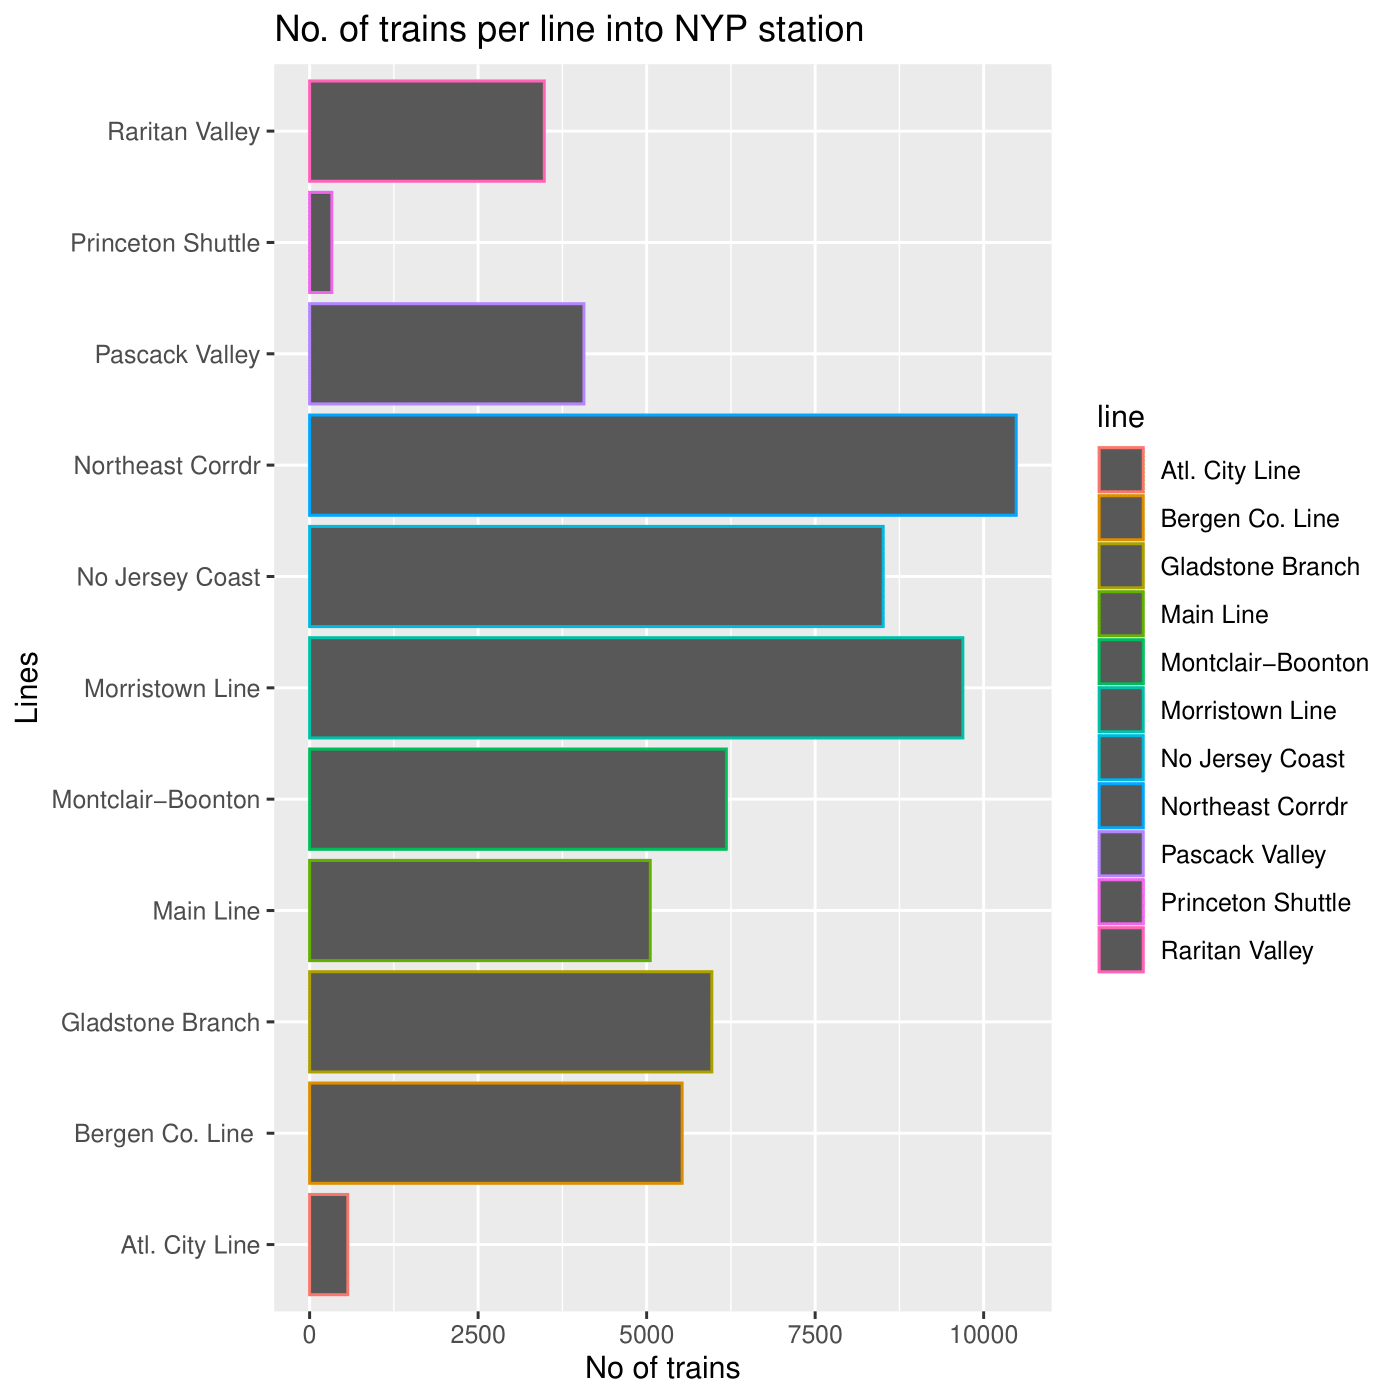
\includegraphics[scale=0.25]{No of lines into NY.png}
    \caption{Bar Chart}
    \label{fig:9}
\end{figure}
\begin{figure}
    \centering
    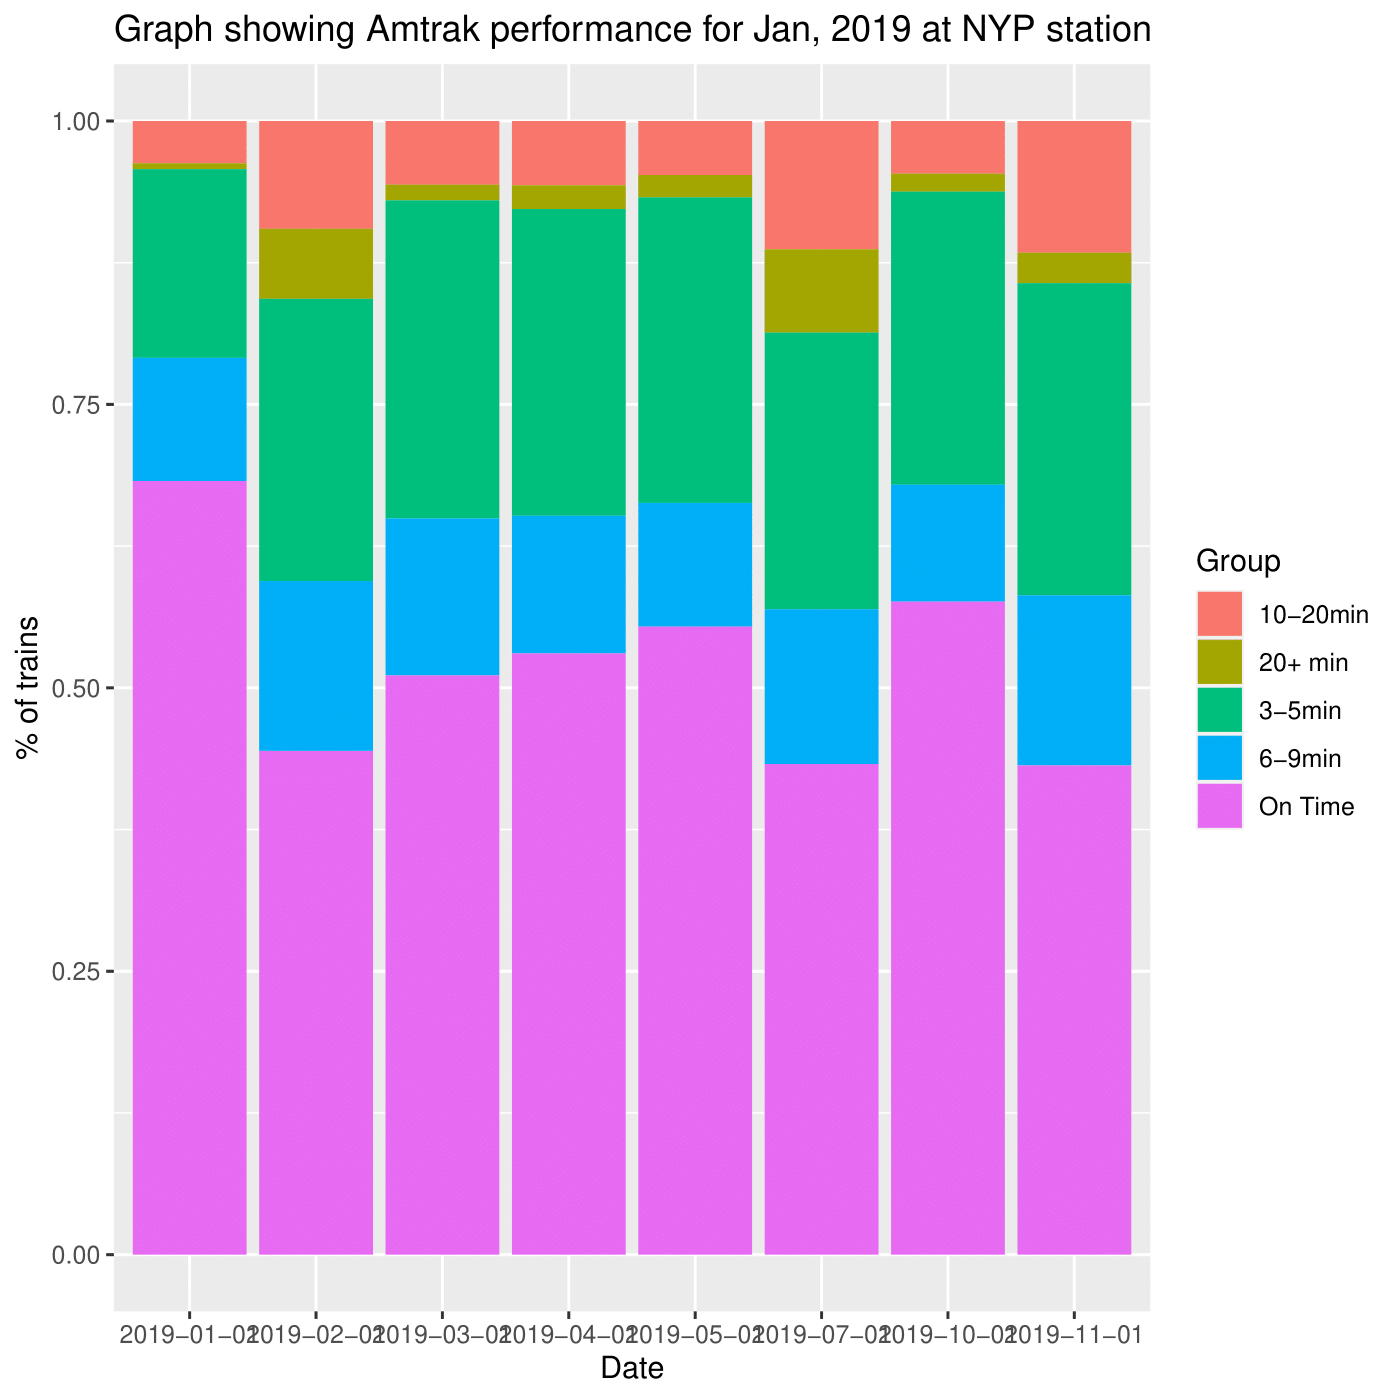
\includegraphics[scale=0.25]{Amtrak Performance.png}
    \caption{Bar Chart}
    \label{fig:10}
\end{figure}
\begin{figure}
    \centering
    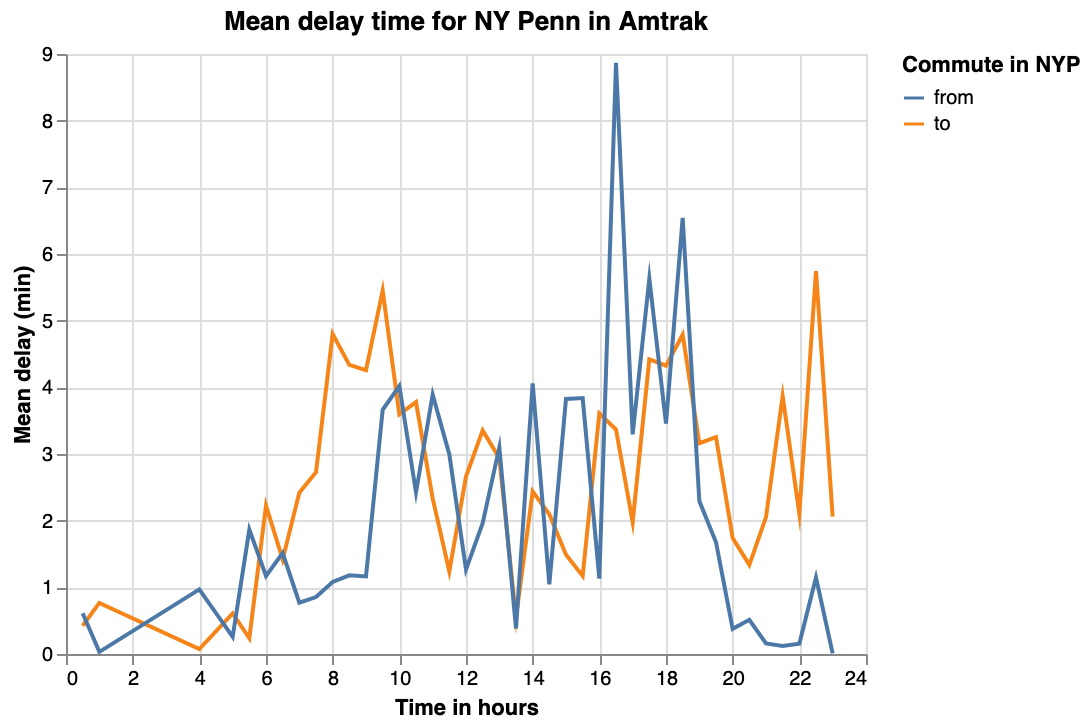
\includegraphics[scale=0.25]{line.png}
    \caption{Line Chart}
    \label{fig:11}
\end{figure}
\begin{figure}
    \centering
    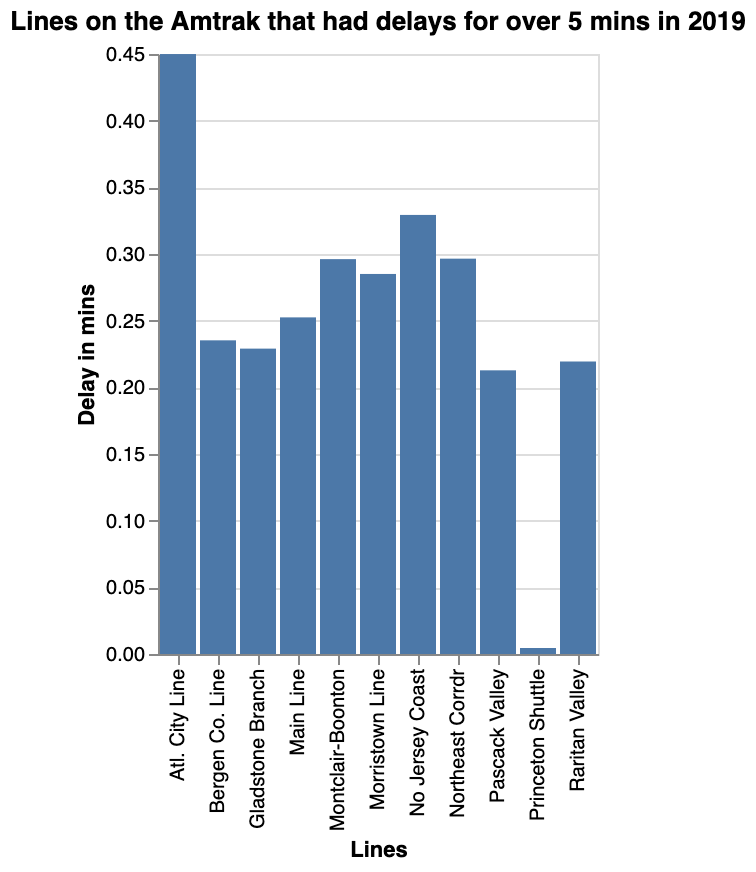
\includegraphics[scale=0.25]{longDelay.png}
    \caption{Bar Chart}
    \label{fig:12}
\end{figure}

\section{Importance of Visualizations}
The combination of maps and charts above allows for easier processing of the data that is available on the Amtrak rail system. Many sources online simply offer tables or other basic structures for sharing Amtrak rail system data. By presenting raw numbers in a visual way, the end user can gain a better understanding of the issue at hand as well as what changes to address these issues should be made. Broadly speaking, presenting data visually leads to better analyses and understanding of important issues, as well as improves decision making~\cite{url2}. In our project specifically, since rail transit is a geospatial issue, integrating both a map and charts harnesses the benefits of data visualization to the specific concerns Amtrak authorities are aiming to address.

\section{Conclusion}
In this dashboard, we have explored various data features related to Amtrak’s rail performance across the nation. With this, we have been able to see that delays, on time performance and congestion at certain stations is a problem that Amtrak needs to address. This project has allowed us to visualize the disparities in rail access across the country, while also revealing that ridership and delays along routes remain concerns that need to be addressed. In keeping with Amtrak’s own 2035 vision for an improved national railroad system, this project offers a way to pinpoint which parts of the country are most in need of improvements. The dashboard has a dual purpose for two types of users. Firstly, the average train rider can get a sense of what delays and congestion to expect when planning their travel. Secondly, Amtrak authorities and employees can use this type of information and visualizations to meet their 2035 goals. At a societal level, access to rail transit should be made more efficient and accessible in all parts of the continental United States, and our dashboard is one way of focusing on certain areas that can contribute to this goal.

%
% the environments 'definition', 'lemma', 'proposition', 'corollary',
% 'remark', and 'example' are defined in the LLNCS documentclass as well.
%

%
% ---- Bibliography ----
%
% BibTeX users should specify bibliography style 'splncs04'.
% References will then be sorted and formatted in the correct style.
%
\bibliographystyle{splncs04}
\bibliography{mybibliography}
%
\end{document}
